% !TeX root = ../solution.tex

\hypertarget{he22.21}{%
\chapter{[HE22.21] Textbook}\label{he22.21}}

\begin{marginfigure}
	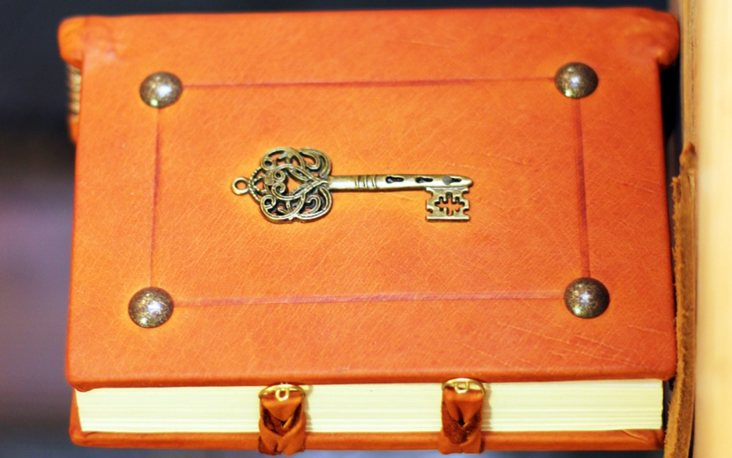
\includegraphics[width=49mm]{level5/challenge21.jpg}
\end{marginfigure}
\subsection{Intro}
I've got the source code and the output of a simple cipher.

\noindent Can you calculate the flag from it?

\noindent File \verb+textbook.zip+.

\subsection{Hint}

As usual, the flag starts with \verb+he2022+.

\section{Solution}\label{hv22.21solution}
The code generator is very simple, each character in the flag is coded as
\verb+pow(ord(c), e, n)+ -- take the ASCII value of the character to the power
$e$ and then store the modulo $n$.  Since we have a crib (``he2022´´) and know
the exponent, we can also calculate the real value of \verb+pow(ord(c),e)+.
Subtract the coded value, we get a number that is known to be a multiple of
$n$, so taking two such numbers, we can calculate $n$ as the GCD of the two
numbers.  Once $n$ is known, we can calculate a rainbow table for all printable
characters and look-up the flag from the encrypted flag:

\begin{minted}{python}
import math

def multi_n(c, cr):
    tmp = pow(ord(c), e)
    return (tmp - cr)

   
with open('output','r') as inF:
    s = inF.read()[1:-2]
    crypt = [int(x) for x in s.split(', ')]

n = math.gcd(multi_n(crib[0], crypt[0]),
            multi_n(crib[1], crypt[1]))

rainbow = {}
for i in range(32,128):
    rainbow[pow(i,e,n)] = chr(i)

res = ''
for i in crypt:
    res += rainbow[i]

print(res)
\end{minted}
Flag \verb+he2022{!!t3xtb00k_crypt0!!}+.
	









